
\section{Método de Monte Carlo y Simulación}
Para introducir el método de Monte Carlo, consideremos el problema de la integración numérica. Existen diversos métodos numéricos para aproximar (computacionalmente) integrales de la forma:
\[\int_{[0,1]^d}f(x)dx,\]
basados en fórmulas del tipo $\sum_{i=1}^n w_if(x_i)$, cuando $f:\,\R^d\rightarrow\R$ es una función conocida y, usualmente, la suma de los términos $w_i$ es uno y los términos $x_i$ son puntos del conjunto $[0,1]^d$. Por ejemplo, $w_i = 1/k$ y la malla de $[0,1]^d$ compuesta por:
\[\left\{0,\frac{1}{k},\frac{2}{k},\cdots,\frac{k}{k}\right\}^d\hspace{1cm}\text{Para algún $k$ natural.}\]
La cual contiene $n = (k+1)^d$ ($\approx k^d $) puntos. Si el método es de orden 1, el error estará asociado al orden del salto de la malla, en este caso es de $1/k$, por lo tanto:
\[error\,\sim\,\frac{1}{k}\approx \frac{1}{n^{1/d}}\]
Luego, si quisiéramos ajustarnos a un error de un orden pequeño, $\varepsilon > 0$, necesariamente tendríamos que tomar una cantidad de datos proporcionalmente, de la forma; $n\,\approx\,1/\varepsilon^d$, lo que es aceptable para un $\varepsilon$ pequeño y un $d$ pequeño (por ejemplo $d\leq 3$). El problema es que para variables de dimensión mayor a eso, el $n$ asociado crece de manera abrupta. \\Los métodos de Monte Carlos ofrecen una alternativa a este problema, reformulando la integral, vista ahora como la esperanza de una variable aleatoria. La discretización se forma de manera natural al elegir $w_i = 1/n$ y $x_i$ como la realización de variables aleatorias uniformes en $[0,1]^d$. Luego, la convergencia de $\sum_{i=1}^n w_if(x_i)$ estará garantizada por la Ley de los Grandes Números.

\begin{teorema}[Ley de los Grandes Números (L.G.N.)] Sean $(X_n)_{n\in\N}$ variables aleatorias $i.i.d.$, con $\E(X_1)=\mu\,<\,+\infty$. Se define el promedio finito:
\[\overline{X}_n\,=\,\frac{1}{n}\sum_{i=1}^nX_i\]
Entonces:
\[\overline{X}_n\,\xrightarrow{\,\,\,n\,\,\,}\,\mu\hspace{1cm}c.s.\text{ y en }L^1\]
\end{teorema}

\begin{obs}
\begin{itemize}
    \item[]
    \item Si $X_1 \in L^p$, entonces la convergencia es en $L^p$.
    \item Si $\sigma^2 = Var(X_1)\,<\,+\infty$, entonces:
    \[\E\left( \left|\overline{X}_n-\mu\right|\right)\,\leq\,\frac{\sigma}{\sqrt{n}}\]
\end{itemize}
\end{obs}
Además de esto, la taza de convergencia es del orden de $n^{1/2}$ y está dada por el Teorema Central del Límite. Claramente, la taza de convergencia podría parecer algo lenta en comparación con las tazas de otros métodos numéricos de integración en dimensión 1. Pero todos esos métodos colapsan cuando nos escapamos a dimensiones mayores.\newline \\
Siguiendo con el ejemplo anterior, llamemos $I$ a la integral que queríamos aproximar:
\[I\,=\,\int_{[0,1]^d}f(x)dx\]
Si definimos la variable $U\sim\,unif([0,1]^d)$, es decir $U=(U_1,U_2,\cdots,U_d)$, con $U_i\sim\,unif(0,1)$ $i.i.d$, entonces la integral anterior la podemos escribir como $I=\E(f(U))$. Considerando $U^{(1)},U^{(2)},\cdots,U^{(m)}$ realizaciones $i.i.d.$ de la variable $U$, por \textbf{L.G.N.}:
\[\frac{1}{m}\sum_{i=1}^m f(U^{(i)})\,\approx\,I\]

\subsection{Descripción del método}
Para usar el método de Monte Carlo, es necesario poder escribir la cantidad de interes como el valor esperado de una variable aleatoria \textit{"eficientemente simulable en un computador"}. Esto suele ser fácil, como es el caso de la aproximación de una integral, pero podría ganar mucha más complejidad, como cuando deseamos resolver alguna ecuación diferencia parabólica o elíptica.\\ \newline
Sea un valor de interés, $\alpha\in\R$, los pasos a seguir son:
\begin{itemize}
    \item[1.] Escribir $\alpha = \E(X)$, donde $X$ es una variable aleatoria.
    \item[2.] Para algún $n$ suficientemente grande, simular $X_1,X_2,\cdots,X_n$ copias $i.i.d$ de $X$ (muestra).
    \item[3.] Aproximar $\alpha\approx\,\frac{1}{n}\sum_{i=1}^nX_i$.
\end{itemize}
Es calro, por \textbf{L.G.N.} que a medida que nuestra muestra aumenta, la estimación será más cercana. Por lo tanto hay que tener una idea de lo que puede ser "suficientemente grande" en cada caso de estimación.\\
Ventajas de $M.M.C$ (método de Monte Carlo):\\
\begin{itemize}
    \item Simple de implementar.
    \item Escala moderadamente bien, a pesar de la dimensión.
\end{itemize}
Desventajas de $M.M.C$:
\begin{itemize}
    \item El resultado es aleatorio (para cada realización diferente, el resultado de la estimación variará).
    \item El error es del orden $1/\sqrt{n}$, lo que en la practica no suele ser muy bueno.
\end{itemize}
\begin{obs} Si $\sigma^2 = Var(X_1)<\infty$, por el \textbf{T.C.L.}:
\[\frac{\overline{X}_n -\alpha}{\sigma / \sqrt{n}}\approx Z,\hspace{1cm}Z\sim\mathcal{N}(0,1)\]
Así,
\[|\overline{X}_n -\alpha| \approx|Z|\frac{\sigma}{\sqrt{n}}\]
Luego, es de utilidad aproximar (estimar) $\sigma$ para tener una idea del error cometido. 
\end{obs}

\begin{ejemplo}
Dada $Y$ variable aleatoria en $\R$ y $A\subseteq\R$. Si me intereza calcular (estimar):
\[p = \pb\left(Y\in A\right) = \E\left(\mathbbm{1}_{Y\in A}\right)\]
Lo natural es definir $X=\mathbbm{1}_{Y\in A}$. Sean $X_1,X_2,\cdots,X_n$ copias $i.i.d.$ de $X$, luego:
\[p\approx \frac{X_1+X_2+\cdots+X_n}{n}=:\hat{p}\]
Notemos que $\sigma^2 = Var(X) = Var(Bernoulli(p)) = p(1-p) \leq 1/4$ (ver figura).
\newline 
\begin{figure}[h!]
    \centering
    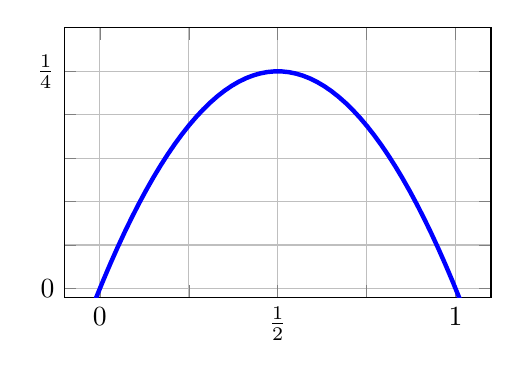
\begin{tikzpicture}
        \begin{axis}[width=7cm, height=5cm,xmin=-0.1,xmax=1.1,ymin=-0.01,ymax=0.3, xmajorgrids=true, ymajorgrids=true, xtick={0,0.25,0.5,0.75,1},  xticklabels={0,,$\frac{1}{2}$,,1}, ytick={0,0.05,0.1,0.15,0.2,0.25}, yticklabels={0,,,,,$\frac{1}{4}$},samples =500]
        \addplot[blue, ultra thick] (x,x-x*x);
        \end{axis}
    \end{tikzpicture}
    \caption{Gráfico de $p(1-p)$, cuyo vértice (punto max) se encuentra en (1/2,1/4)}
\end{figure}\\
Supongamos que queremos un intervalo de confianza al $95\%$, con error $\pm\varepsilon$.
\[0.95 \,\overset{!}{=}\,\pb\left(p\in[\hat{p}-\varepsilon\,,\,\hat{p}+\varepsilon]\right)= \pb\left(|\hat{p}-p|\leq\varepsilon\right) = \pb\left(\frac{|\hat{p}-p|}{\sigma/\sqrt{n}} \leq \frac{\varepsilon\sqrt{n}}{\sigma}\right)\]
Nuevamente, ocupando \textbf{T.C.L.}:
\[0.95\approx \pb\left(|\mathcal{N}(0,1)|\leq \frac{\varepsilon\sqrt{n}}{\sigma}\right)\,\Rightarrow
\,\frac{\varepsilon\sqrt{n}}{\sigma}\approx\,1.96\]
\[\Rightarrow\,\,\sqrt{n}\approx\,\frac{1.96\sigma}{\varepsilon}\,\,\Rightarrow\,\,n\approx\,\frac{1.96^2\sigma^2}{\varepsilon^2}\leq\frac{4\cdot 1/4}{\varepsilon^2}=\frac{1}{\varepsilon^2}\]
Así, ganamos una relación entre la cantidad de muestra que necesitamos para controlar el error asociado a la estimación. Por ejemplo, si queremos un error no mayor a $\varepsilon = 0.01$, bastaría con tomar $n=10000$ observaciones para lograrlo con $95\%$ de confianza.
\end{ejemplo}

\subsection{Simulación de variables aleatorias}
En la actualidad, todos los lenguajes de programación modernos poseen generadores de números \textit{pseudoaleatorios}\footnote{La palabra marca una diferencia respecto al término $aleatorio$, pero no se dará enfoque a este concepto en este curso.}. Tales programas producen como salida, una secuencia perfectamente determinista (y, a veces, periódica), pero cuyas propiedades estadísticas se parecen lo suficiente a las de una secuencia de realizaciones independientes de una variable aleatoria $unif(0,1)$. El problema de crear un "buen generador" de números aleatorios es crear una fórmula de recurrencia que, en un tiempo razonable, produzca una secuencia de números que se parezca lo más posible a una secuencia de realizaciones independientes $unif(0,1)$ con el periodo lo más largo posible.\footnote{ver  \cite[cap. 1]{Pard}}\\ Con este recurso computacional en mente, el objetivo ahora es recrear otras variables aleatorias con distribuciones diferentes que sean de interés, a partir de realizaciones uniformes en el intervalo $(0,1)$.\\ \newline
\begin{enumerate}
    \item \textbf{Simulación de una variable aleatoria Bernoulli:} Sea $0<p<1$. Si $U$ es una variable aleatoria $unif(0,1)$. Entonces $X=\mathbbm{1}_{\{U \leq p\}}$ es una variable $Bernoulli$ de parámetro $p$.
    \item \textbf{Simulación de una variable aleatoria Binomial:} Sea $n\in\N$, $U_1,U_2,\cdots,U_n$ variables aleatorias $i.i.d.$ $unif(0,1)$, entonces:
    \[X=\mathbbm{1}_{\{U_1\leq p\}} + \mathbbm{1}_{\{U_2\leq p\}}+\cdots + \mathbbm{1}_{\{U_n \leq p\}}\]
    es una variable aleatoria binomial de parámetros $n$ y $p$, $B(n,p)$.
    \item \textbf{Simulación de una variable aleatoria Geométrica:}
    \[X = \inf\{k\geq 1;\,U_k\leq p\}\]
    Cuando $(U_n)_n$ son variables aleatorias $i.i.d.$ con distribución $unif(0,1)$, \\entonces $X\sim geom(p)$.
\end{enumerate}
Para proceder a una simulación más eficiente nos basaremos en el siguiente lema.

\begin{lem} Sea $X$ una vaiable aleatoria, y $F$ su función de distribución ($i.e.$ $F(x) = \pb(X\leq x)$). Para $0\leq t\leq 1$, definimos:
\[F^{-1}(t) = \inf\{x;\,F(x)>t\}\]
Entonces, si $U$ tiene ley $unif(0,1)$, $F^{-1}(U)$ tiene ley $\mathcal{L}(X)$.
\end{lem}

\textbf{Demostración: }Notemos que si $F$ es una función invertible, entonces su inversa coincide con $F^{-1}$, además tendremos que $F^{-1}$ será una función creciente, al igual que $F$. Entonces:
\[\pb(F^{-1}(U)\leq t) = \pb(U\leq F(t)) = \int_{0}^{F(t)}dx = F(t) = \pb(X\leq t)\]
Donde la integral sale del hecho de que $U$ es una variable uniforme entre $[0,1]$ y $F(t)$ siempre pertenece a tal intervalo por ser una probabilidad.\\ \newline
¿Qué pasa cuando la función $F$ no es invertible? Notemos que $\forall\,x\in\R$:
\begin{equation}
    \{t\,:\,F^{-1}(t)\leq x\}\,\cup\,\{F(x)\}\,=\,\{t\,:\,t\leq F(x)\}
    \label{eq.dem1MC}
\end{equation}
En efecto: claramente $F(x)\in\,\{t\,:\,t\leq F(x)\}$, además:
\[F^{-1}(t)\leq x\,\Longleftrightarrow\,\inf\{y\,:\,F(y)>t\}\leq x\,\Longleftrightarrow\,\exists y*\leq x,\,\exists y_n\searrow y*,\,t.q.\,F(y_n)>t\,\forall\,n\]
Dado que $F$ es una función de distribución, es contínua por la derecha, entonces $F(y*)\geq t$. Ocupando que $F$ es creciente, tenemos:
\[y*\leq x\,\wedge\,F(y*)\geq t\,\Rightarrow\,F(x)\geq F(y*)\geq t\]
Esto prueba la inclusión $\subseteq$ en \ref{eq.dem1MC}. Recíprocamente, si $F(x)\geq t$ hay dos casos posibles:
\begin{itemize}
    \item Si $t=F(x)$, entonces el lado izquierdo de \ref{eq.dem1MC} corresponde al síngleton.
    \item Si $t<F(x)$, por definición de ínfimo:
    \[x\geq \inf\{y\,:\,F(y)>t\} = F^{-1}(t)\]
    Por lo tanto $t$ pertenece al lado izquierdo de \ref{eq.dem1MC} y se concluye la segunda inclusión.
\end{itemize}
Entonces, usando \ref{eq.dem1MC}; sea $Y=F^{-1}(U)$:
\[\pb(Y\leq y) = \pb(F^{-1}(U)\leq y)\]
Como $U$ es una variable aleatoria absolutamente contínua los síngleton tienen medida de probabilidad igual a cero. Así:
\[\pb(F^{-1}(U)\leq y) = \pb(F^{-1}(U)\leq y\,\vee\,U=F(y))\, \overset{\ref{eq.dem1MC}}{=}\,\pb(U\leq F(y)) = F(y)\]
Luego la función de probabilidad acumulada de $Y$ es $F$, es decir $Y\sim \mathcal{L}(X)$. \rule{0.7em}{0.7em}\\ \newline
En los casos en que la función de distribución $F$ tiene inversa de forma explícita, el lema anterior nos permita, cómodamente, simular realizaciones de la variable $X$.

\begin{ejemplo}[variable aleatoria exponencial.] Para $X\sim exp(\lambda)$, $F(x)=1-e^{-\labda x}$ $\forall\,x\geq 0$, luego:
\[F^{-1}(t) = -\frac{log(1-t)}{\lambda}\]
Por el lema anterior; para $U\sim unif(0,1)$.
\[F^{-1}(U) = -\frac{log(1-U)}{\lambda}\,\sim\,exp(\lambda)\]
Finalmente, si $U\sim unif(0,1)$ entonces la variable aleatoria $1-U$ también es uniforme en el intervalo [0,1], por lo tanto:
\[F^{-1}(U)\,\overset{d}{=}\,-\frac{log(U)}{\lambda}\,\sim\,exp(\lambda)\]
\end{ejemplo}

Una de las variables más importantes de simular son las variables aleatorias normales. Lamentablemente, el lema anterior no nos es de utilidad pues no conocemos una forma explícita de la función de distribución, sin embargo podemos hacer lo siguiente.\\ Si $U,V\,\sim unif(0,1)$ independientes, entonces:
\[X:= \sqrt{-2log(U)}cos(2\pi V)\hspace{0.3cm},\hspace{0.3cm}Y:=\sqrt{-2log(U)}sin(s\pi V)\]
son variables aleatoria con distribución $\mathcal{N}(0,1)$ independientes (\textbf{ejercicio, cambio de variable}). Luego, para generar $\mathcal{N}(\mu,\sigma^2)$, basta ponderar y trasladar de la forma $\sigma X + \mu$.\footnote{Los software ocupan algoritmos de mayor eficiencia para generar variables aleatorias normales, por ejemplo el algoritmo de Ziggurat.}

\subsection{Método de Aceptación-Rechazo}
Supongamos que conocemos $X$, una variable aleatoria con función de densidad $f$ conocida, pero sin $F^{-1}$ explícita. El objetivo es poder simular realizaciones de $X$, ¿cómo podemos simular $X$?\\ Supongamos que existe $Y$, una variable aleatoria eficientemente simulable, con función de densidad $g$ que cumpla lo siguiente:
\[\exists\,k>0,\hspace{0.5cm}f(x)\leq kg(x)\,\,\forall\,x\]
\[g(x)>0\,\Longleftrightarrow\,f(x)>0\]
Entonces, $\forall\,x$ tal que $g(x)>0$, definimos:
\begin{equation}
    \alpha(x) = \frac{f(x)}{kg(x)}
    \label{eq.alpha de x}
\end{equation}

\begin{prop} Sean $(Y_n,U_n)_n$ una secuencia de realizaciones independientes, tal que $U_n\sim unif(0,1)$, $Y_n\,\overset{d}{=}\,Y$ y $U_n$ es independiente de $Y_n$ para todo $n$. Definimos la variable aleatoria $N$ como:
\[N=\inf\{k\in\N\,:\,U_k \leq \alpha(Y_k)\}\]
Entonces $N<\infty$ c.s. y $Y_N \,\overset{d}{=}\,X$.
\end{prop}

\textbf{Demostración: }Veamos que $N<\infty$ $\pb-c.s.$ Para ello, notemos que:
\[\pb(N=\infty) = \pb(\forall\,m\,,\,U_m>\alpha(Y_m)) = \lim_{n \to \infty}\pb(\forall\,m=1,\cdots,n\,:\,U_m>\alpha(Y_m))\]
Como las realizaciones son $i.i.d.$ tenemos que:
\[\lim_{n \to \infty}\pb(\forall\,m=1,\cdots,n\,:\,U_m>\alpha(Y_m)) = \lim_{n \to \infty}\left[\pb(U_m > \alpha(Y_m))\right]^{n} = 0\]
Donde la última igualdad sale de que $\pb(U>\alpha(Y)) < 1$ (con la desigualdad estricta.\\ \newline
En efecto, sea $p=\pb(U\leq \alpha(Y))$, usando probabilidades totales:
\[p = \pb(U\leq \alpha(Y)) = \int_{\R}\pb(U\leq \alpha(y))g(y)dy= \int_{\R}\left(\int_{0}^{\alpha(y)}dx\right)g(y)dy\]
\[=\int_{\R}\alpha(y)g(y)dy = \int_{\R}\frac{f(y)}{kg(y)}g(y)dy = \frac{1}{k}\int_{\R}f(y)dy = \frac{1}{k}\,>\,0\]
Como $p>0$,entonces $1-p = \pb(U>\alpha(Y))<1$ y concluímos que $N<\infty$ $\pb-c.s.$\\ \newline
Ahora veamos que $Y_N \,\overset{d}{=}\,X$. $\forall\,A\subseteq \mathcal{B}(\R)$ tenemos que:
\[\pb(Y_N \in A) = \sum_{n=1}^{\infty}\pb(Y_n \in A,\,N=n) = \sum_{n=1}^{\infty}\pb(Y_n \in A,\,U_n\leq\alpha(Y_n),\,U_m>\alpha(Y_m),\,\forall\,m=1,\cdots,n-1)\]
\[=\sum_{n=1}^{\infty}(1-p)^{n-1}\pb(Y_n \in A,\,U_n\leq \alpha(Y_n))\]\[= \sum_{n=1}^{\infty}(1-p)^{n-1} \int_{\R}\pb(y \in A,\,U_n\leq \alpha(y))g(y)dy\]
Recordando que $U_n$ es uniforme, y (por lo visto al principio de la demostración) $p=1/k$:
\[\pb(Y_N \in A)= \sum_{n=1}^{\infty}(1-p)^{n-1} \int_{\R}\pb(y \in A,\,U_n\leq \alpha(y))g(y)dy\]\[= \sum_{n=1}^{\infty}(1-p)^{n-1}\int_{\R}\mathbbm{1}_{y\in A}\alpha(y)g(y) dy\]
\[=\sum_{n=1}^{\infty}(1-p)^{n-1}\int_{\R}\mathbbm{1}_{y\in A}\frac{f(y)}{kg(y)}g(y) dy\] \[= \sum_{n=1}^{\infty}(1-p)^{n-1}p\int_{\R}\mathbbm{1}_{y\in A}f(y) dy\] \[= \pb(X \in A)\sum_{n=1}^{\infty}p(1-p)^{n-1}= \pb(X\in A)\] 
\rule{0.7em}{0.7em}\\

Entonces, definiendo $\alpha(x) = \frac{f(x)}{kg(x)}$ para todo $x$ tal que $g(x)>0$. Explicamos el método de Aceptación-Rechazo mediante el siguiente algoritmo:\\ \newline
\textbf{Algoritmo Aceptación-Rechazo:} para simular la variable $X$.
\begin{enumerate}
    \item Simular $U\sim unif(0,1)$, simular $Y\sim g$. Ambas ($U$ e $Y$) independientes entre si.
    \item Si $U\leq \alpha(Y)$, $X=Y$ es un muestreo de $X$.
    \item Si $U> \alpha(Y)$, volver al paso 1 e iterar.
\end{enumerate}
\newline
\textbf{Observación: }De la demostración previa notamos que; $N\sim geom(1/k)$. Entonces el valor esperado de la cantidad de iteraciones necesarias para simular un valor de $X$ es $\E(N) = k$. Luego, para que el método termine en un tiempo razonable, es necesario ajustar el valor $k$ lo más cercano a 1 posible, es decir; elegir una densidad $g$ suficientemente parecida a $f$.\\ \newline
\textbf{Observación: }El método anterior es válido, aún tomando densidades con respecto a una medida $\mu$ cualquiera. Es decir, para $f$ y $g$ densidades de $X$ e $Y$, respectivamente, que cumplen las condiciones:
\[\prob\left(X\in A\right) = \int_{A}f(x)\mu(dx) \leq \int_{A}kg(x)\mu(x) = k\prob\left(Y\in A\right)\]
En particular, si $X$ es una variable aleatoria discreta, digamos en $\N$, entónces $f(x) = \prob(X=x)$ es la densidad de $X$ con respecto a la medida \textit{cuenta-puntos}. Luego, si $Y$ es otra variable aleatoria discreta que cumple las hipótesis con su densidad, es posible aplicar el método.

\subsection{Reducción de varianza}
Recordemos que el método de Monte Carlo (M.M.C.) aproxima un valor
\begin{equation}
    \alpha = \E(X) \approx \frac{1}{n}\sum_{i=1}^{n}X_i
    \label{redvar_1}
\end{equation}
donde $X_1,\cdots,X_n$ son copias $i.i.d.$ de $X$. Además sabíamos que el error es del orden de
$\frac{\sigma}{\sqrt{n}}$, con $\sigma^2 = Var(X)$.\\
Notamos que el valor por estimar en $\ref{redvar_1}$ sólo depende de la esperanza de la variable $X$ y no en la variable en sí o su distribución, por lo tanto tenemos la libertad de cambiar la variable a utilizar por una que tenga menor varianza, así estimaremos el mismo valor con un error menor.

\subsubsection{Muestreo preferencial}
Sea $X$ con densidad $f$. Sea el valor a estimar
\[\alpha = \E(g(X))\]
donde $g:\R\rightarrow\R$ es una función dada.\\ \newline
Ahora, supongamos que tenemos $Y$, otra variable aleatoria con densidad $\Tilde{f}>0$, entonces:
\[\alpha = \E(g(X)) = \int g(x)f(x) dx = \int \frac{g(x)f(x)}{\Tilde{f}(x)}\Tilde{f}(x) dx \]
Si definimos la función $h$ como:
\[h(x) = \frac{g(x)f(x)}{\Tilde{f}(x)}\]
Entonces $\alpha$ es la esperanza de la función $h$ bajo la densidad $\Tilde{f}$, es decir $\alpha = \E(h(Y))$. Además:
\[Var(h(Y)) = \E\left(h(Y)^2\right) - \alpha^2\]
\[= \int \frac{g(x)^2f(x)^2}{\Tilde{f}(x)^2}\Tilde{f}(x)dx - \alpha^2\]
\[= \int \frac{f(x)^2g(x)^2}{\Tilde{f}(x)}dx - \alpha^2\]
Si $g\geq 0$, entonces si escogemos \begin{equation}
    \Tilde{f}(x) = \frac{g(x)f(x)}{\alpha}
    \label{eq.rv2}
\end{equation}
entonces, obtenemos $Var(h(Y)) = 0$.\\ Evidentemente, \ref{eq.rv2} no funciona en la práctica, pues no conocemos el valor de $\alpha$. Sin embargo, nos sugiere que sería óptimo tomar una función $\Tilde{f}$ suficientemente parecido, en cuanto a forma, a $g(x)f(x)$ (diferenciado por una pondderación constante).\\ \newline

Esto motiva el siguiente procedimiento heurístico, escogeremos $\Tilde{f}$ cumpliendo:
\begin{itemize}
    \item $\Tilde{f}(x)$ "parecido" a $|g(x)f(x)|$, normalizado para que integre 1.
    \item Sea fácil de simular una variable $Y$, con densidad $\Tilde{f}$.
\end{itemize}
Luego basta aproximar $\alpha \approx \frac{1}{n}\sum_{i=1}^n h(Y_i)$, con $Y_1,\cdots,Y_n$ copias $i.i.d.$ de $Y$.\\ \newline

\textbf{Ejemplo: }Queremos aproximar:
\[I = \int_{0}^1 cos\left(\frac{\pi x}{2}\right)dx = \frac{2}{\pi}\]
Suponiendo que no podemos calcular esta integral, difiniendo:
\[I = \E(g(X)),\hspace{1cm}g(x) = cos\left(\frac{\pi x}{2}\right)\]
con $X$ una variable aleatoria uniforme en el intervalo $[0,1]$, podemos calcular $I$ mediante $M.M.C.$.\\ \newline
En este caso, podríamos reemplazar la función $coseno$ por un polinomio de grado 2. Dado que el interior de la integral es 0 en $x=1$ y 1 en $x=0$, es natural elegir $\Tilde{f}(x)$ de la forma $\lambda(1-x^2)$. Si normalizamos la función en este intervalo, tenemos que $\Tilde{f}(x) = 3(1-x^2)/2$. Al calcular las varianzas, podemos notar que el método reduce la varianza en un factor de 100. \\

\begin{figure}[h!]
    \centering
    \begin{tikzpicture}
        \begin{axis}[width=7cm, height=5cm,xmin=-0.1,xmax=1.1,ymin=-0.01,ymax=1.7, xmajorgrids=true, ymajorgrids=true, xtick={0,0.25,0.5,0.75,1},  xticklabels={0,,,,1}, ytick={0,0.25,0.5,0.75,1,1.25,1.5}, yticklabels={0,,,,1,,1.5},samples =500]
        \addplot[blue, ultra thick] (x,1.5-1.5*x*x);
        \addplot[red, ultra thick](x,cos(deg(1.5707*x)));
        \end{axis}
    \end{tikzpicture}
    \caption{En rojo la función $cos(\pi x/2)$, en azul la función $3(1-x^2)/2$ mayorándola.}
\end{figure}\\

\subsubsection{Variable de control}
Este método involucra escribir $\E(f(X))$ de la forma:
\[\E\left(f(X)\right) = \E\left(f(X)-h(X)\right) + \E\left(h(X)\right)\]
Donde $\E\left(h(X)\right)$ puede ser calculado explícitamente, y $Var\left(f(X)-h(X)\right)$ es significatívamente menor que $Var\left(f(X)\right)$. Así, empleamos el método de Monte Carlo para el cálculo de $\E\left(f(X)-h(X)\right)$ y el cálculo directo de $\E\left(h(X)\right)$.\\ \newline
\textbf{Ejemplo: }Sumpogamos que deseamos calcular la siguiente integral:
\[I = \int_{0}^1 e^x dx = e-1\]
Aplicando el $M.M.C.$, con $I=\E(e^X) = \E(g(X))$, con $X\sim unif(0,1)$. Notamos que la varianza de la función es $Var(g(X)) \approx 0,242$.\\
Dado que, cerca de $x=0$, $e^x \approx 1+x$, podemos escribir:
\[\int_{0}^1 e^x dx = \int_{0}^1 (e^x -1-x)dx + \frac{3}{2}\]
En este caso, elegimos $h(x)=1+x$. Es fácil comprobar que $Var\left(g(x)-h(x)\right) \approx 0.0437$. Es decir, hemos reducido la varianza de la estimación en un factor de $5.5$ aproximadamente.

\subsubsection{Variables antitéticas}
Supongamos que deseamos calcular la siguiente integral;
\[I =   \int_{0}^1 f(x)dx\]
Dado que el cambio de variable: $x\rightarrow 1-x$ es invariante ante la medida $dx$ en $[0,1]$. Es decir,
\[\int_{0}^1f(x)dx = \int_{0}^1f(1-x)dx\]
Entonces es posible reescribir $I$ de la sigueinte forma:
\[I = \frac{1}{2}\int_{0}^1 (f(x) + f(1-x))dx\]
Otra forma de plantear el problema, es definir la variable aleatoria $X\sim unif(0,1)$. Así, $1-X \sim unif(0,1)$, entonces:
\[I = \E(f(X)) = \E\left(\frac{f(X)+f(1-X)}{2}\right)\]
y obtenemos la misma conclusión.\\ \newline

Ahora, podemos calcular $I$ con $M.M.C.$. Simulamos $n$ variables aleatorias $i.i.d.$ uniformes en $[0,1]$, $U_1,\cdots,U_n$, y aproximamos $I$ por:
\[I_{2n} = \frac{1}{n}\left(\frac{1}{2}(f(U_1)+f(1-U_1))+ \cdots + (f(U_n)+f(1-U_n))\right)\]
\[= \frac{1}{2n}(f(U_1)+f(1-U_1) + \cdots + f(U_n) + f(1-U_n))\]
A grandes razgos, este método es equivalente a emplear el método tradicional de Monte Carlo, con la variable $\frac{f(U)+f(1-U)}{2}$. Podemos observar que su varianza:
\[Var\left(\frac{f(U)+f(1-U)}{2}\right) = \frac{1}{4}Var\left(f(U) + f(1-U)\right)\]
\[= \frac{1}{4}\left(Var\left(f(U)\right) + 2Cov\left(f(U),f(1-U)\right) + Var\left(f(1-U)\right)\right)\]
Dado que $X\overset{d}{=}1-X$:
\[Var\left(\frac{f(U)+f(1-U)}{2}\right) = \frac{1}{2}\left[Var(f(U)) + Cov(f(U),f(1-U))\right]\]
Así, si $Cov(f(U),f(1-U)) \leq 0$, se reduce la varianza de la estimación en al menos un factor de 1/2.\\ \newline
En general, tenemos que la aproximación mejora siempre que:
\[\E\left(f(U)f(U-1)\right) < \E\left(f(U)^2\right)\]

\begin{lem} Si $f$ es una función \textit{monótona}, entonces:
\[Cov(f(U),f(1-U)) \leq0\]
\end{lem}
\subsubsection{Método de Estratificación}
Este método es bien conocido en el diseño de muestras de encuestas. Supongamos que se busca calcular
\[I = \E\left(g(X)\right) = \int g(x)f(x)dx\]
Donde $X$ tiene ley $f(x)dx$. Consideremos $D_1,\cdots,D_m$, una partición del soporte de la densidad $f$. Luego, podemos descomponer $I$ en
\begin{equation}
    I = \sum_{i=1}^m I_i = \sum_{i=1}^m \E\left(\mathbbm{1}_{\{X\in D_i\}}g(X)\right)
    \label{eq_estrat1}
\end{equation}

Este método propone estimar $I_i$ con $M.M.C.$, usando $n_i$ simulaciones. Definimos como $\sigma_i^2 = Var(\mathbbm{1}_{\{X\in D_i\}}g(X))$. Entonces, la varianza de la aproximación es

\begin{equation}
    \sum_{i=1}^m \frac{\sigma_i^2}{n_i}
    \label{eq_estrat2}
\end{equation}

Si minimizamos \ref{eq_estrat2}, bajo la restricción de un número de simulaciones $\sum_{i=1}^m n_i = n$ dado, obtenemos $n_i =n\sigma_i/\sum_{i=1}^m\sigma_i$, con un valor mínimo de la varianza de
\[\frac{\left(\sum_{i=1}^m \sigma_i\right)^2}{n}\]
Puede probarse que esta varianza es menor que la obtenida con $n$ simulaciones bajo el método estándar de Monte Carlo directamente en \ref{eq_estrat1}. Por supuesto, rara vez es posible calcular el valor de $\sigma_i$, lo que limita el uso de esta técnica (pero bien uno puede estimarlos vía su estimador insesgado de varianza mínima $\frac{1}{n-1}\sum (x_i-\Bar{x})^2$, o bajo el propio $M.M.C.$).
